\documentclass[11pt]{article}
\usepackage[utf8]{inputenc}
\usepackage{amsmath,amssymb}
\usepackage{graphicx}
\usepackage{hyperref}

\title{Sparse Attention Priors for Long-Context Retrieval}
\author{A. Researcher \and B. Collaborator}
\date{\today}

\begin{document}
\maketitle

\begin{abstract}
In this paper we present a method that is used for the purpose of improving retrieval
over very long documents. It is shown by our experiments that the method is effective
and that it can be applied to many different kinds of tasks in a way that is general.
\end{abstract}

\section{Introduction}
\label{sec:intro}
Retrieval-augmented models~\cite{lewis2020rag} struggle when the evidence is spread
across documents that exceed the context window of the reader. Prior work on sparse
transformers~\cite{child2019sparse} reduces the quadratic cost of attention, but does not
address where to look.

We make two contributions. First, we propose a sparse attention prior (Section~\ref{sec:method}).
Second, we evaluate it on three long-context benchmarks (Section~\ref{sec:results}),
see Figure~\ref{fig:overview} for an overview.

\begin{figure}[t]
  \centering
  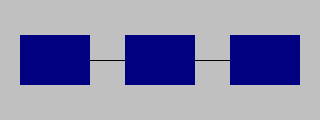
\includegraphics[width=0.8\linewidth]{figures/overview}
  \caption{Overview of the retrieval pipeline with the sparse prior.}
  \label{fig:overview}
\end{figure}

\section{Method}
\label{sec:method}
Let $q$ be a query and $D = \{d_1, \dots, d_n\}$ a set of passages. We define the prior
\begin{equation}
  \label{eq:prior}
  p(d_i \mid q) \propto \exp\big(\lambda \, s(q, d_i)\big),
\end{equation}
where $s$ is a sparse lexical score and $\lambda$ a temperature.

\subsection{Training}
We train the reader with the prior in Eq.~\eqref{eq:prior} fixed, following~\cite{izacard2021fid}.
% TODO: add hyperparameters


\section{Results}
\label{sec:results}
Table~\ref{tab:main} summarises recall@10 across the three benchmarks. Our prior
improves over dense retrieval~\cite{karpukhin2020dense} on every split.

\begin{table}[t]
  \centering
  \caption{Recall@10 on long-context benchmarks.}
  \label{tab:main}
  \begin{tabular}{lccc}
    \hline
    Method & NQ-Long & QASPER & GovRep \\
    \hline
    Dense  & 61.2 & 48.9 & 39.4 \\
    Ours   & \textbf{67.8} & \textbf{55.1} & \textbf{44.0} \\
    \hline
  \end{tabular}
\end{table}

\section{Conclusion}
\label{sec:conclusion}
We introduced sparse attention priors. Future work will explore multilingual corpora.

\bibliographystyle{plain}
\bibliography{refs}
\end{document}
